% FILIPPO
% 2. PLP. The customer can:
%     a. Select multiple product items;
%     b. Add the selected products to the shopping cart;
%     c. Navigate to the shopping cart page;

\subsection{UC7 - Selezione ordinamento dei prodotti nella PLP} \label{UC7}

\begin{figure}[H]
    \centering
    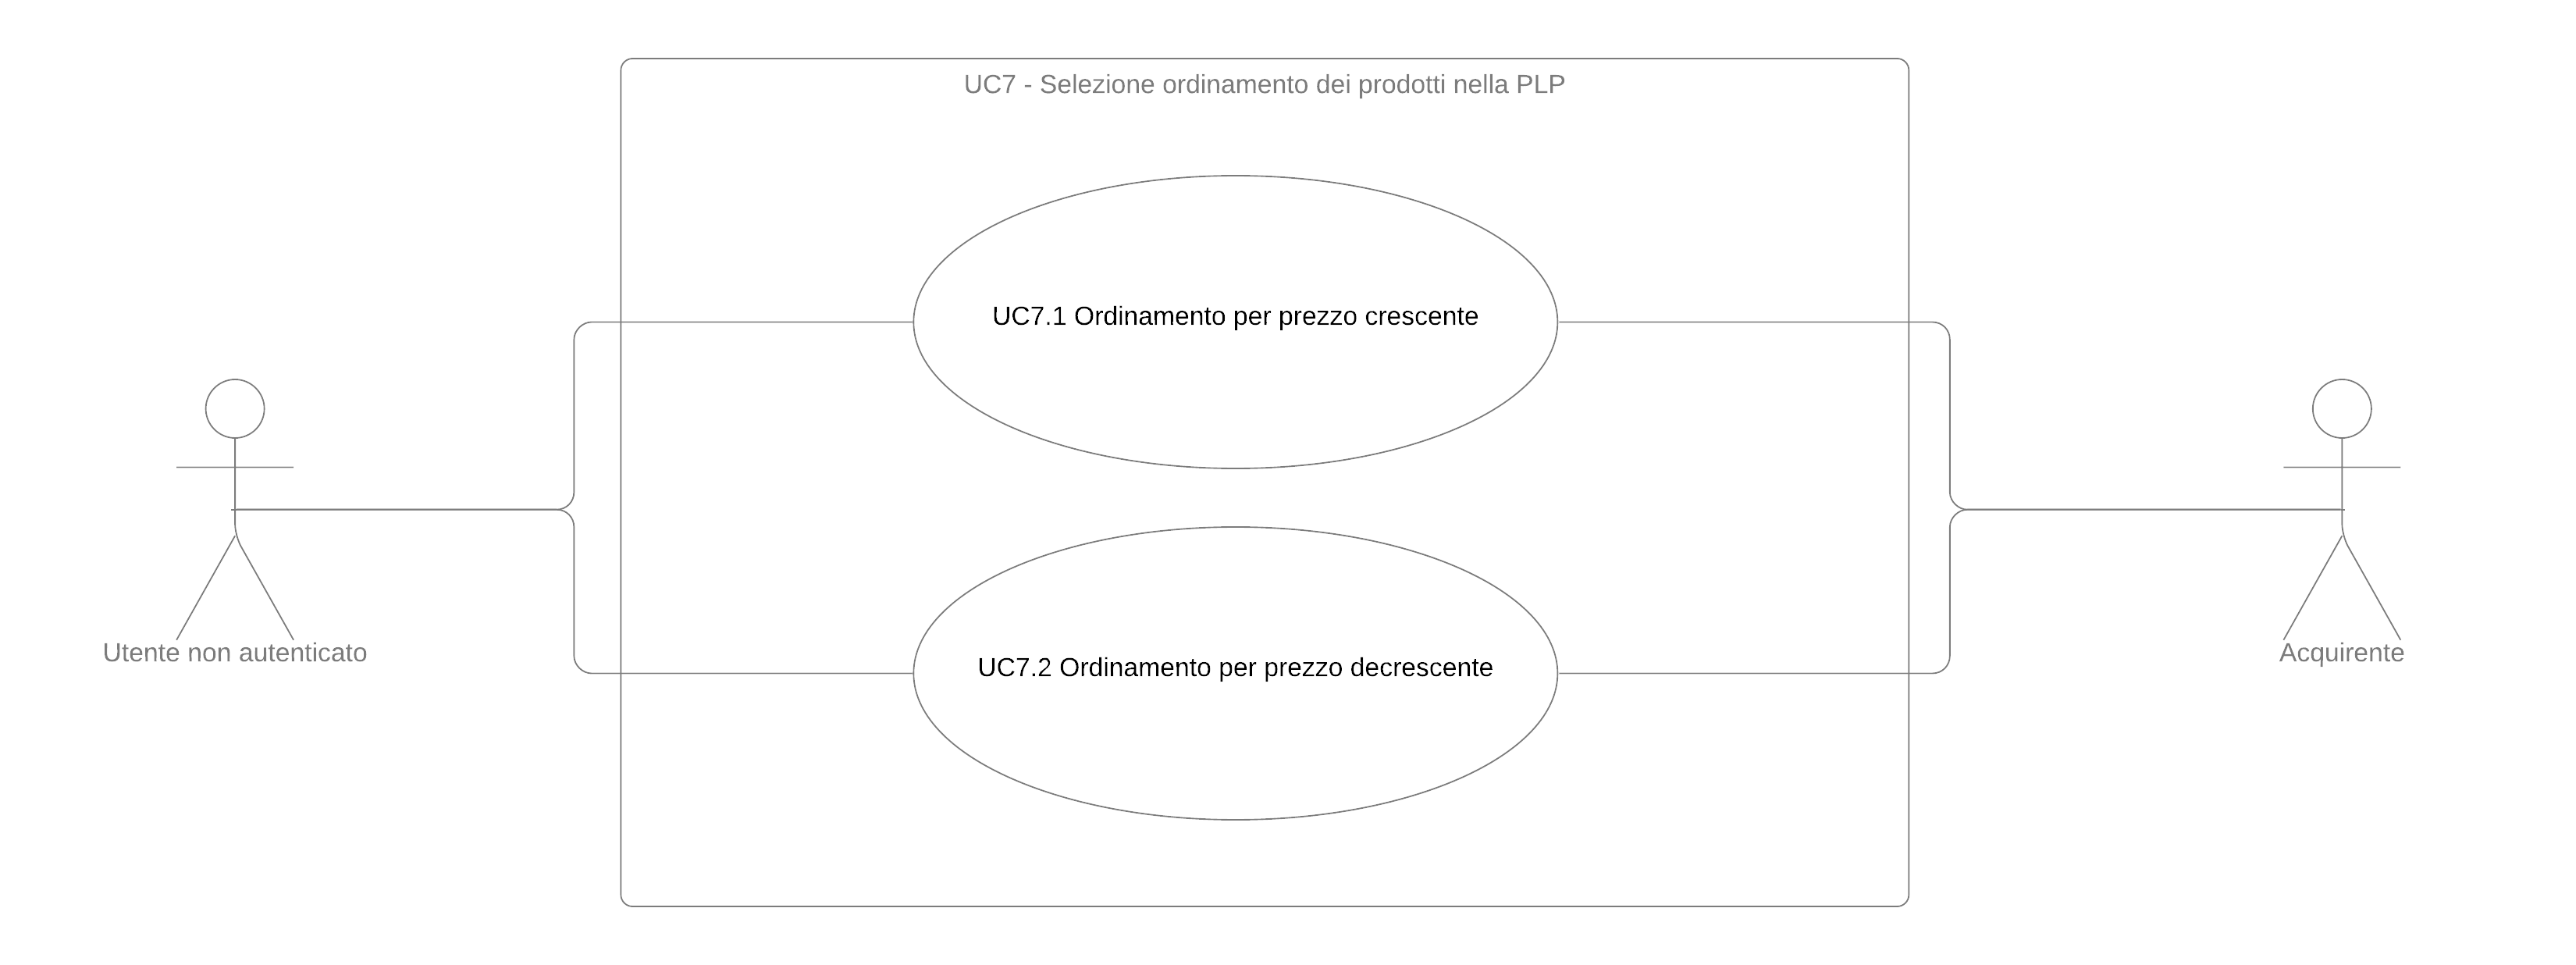
\includegraphics[width=\textwidth]{Immagini/DiagrammiUC/UC7Ordinamento.png}
    \caption{Diagramma di UC7: Ordinamento dei prodotti nella PLP} 
    \label{fig:Checkout}
\end{figure}

L'utente non autenticato o l'acquirente può ordinare i prodotti risultanti dalla ricerca effettuata in precedenza, selezionando uno ed uno solo dei possibili ordinamenti.
\begin{itemize}
    \item \textbf{Attori Primari:} Acquirente; Utente non autenticato.
    \item \textbf{Precondizione:} L'attore è nella PLP e ha selezionato uno degli ordinamenti messi a disposizione.
    \item \textbf{Postcondizione:} I prodotti nella PLP sono ordinati in base all'ordinamento selezionato.
    \item \textbf{Scenario Principale:} L'attore seleziona uno tra i seguenti ordinamenti:
    \begin{itemize}
        \item (UC7.1) - Ordinamento per prezzo crescente.
        \item (UC7.2) - Ordinamento per prezzo decrescente.
    \end{itemize}
\end{itemize}

\subsubsection{UC7.1 - Ordinamento per prezzo crescente} \label{UC7.1}
I prodotti nella PLP vengono ordinati in ordine di prezzo crescente.
\begin{itemize}
    \item \textbf{Attori Primari:} Acquirente; Utente non autenticato.
    \item \textbf{Precondizione:} L'attore è nella PLP e ha selezionato l'ordinamento per prezzo crescente.
    \item \textbf{Postcondizione:} I prodotti nella pagina vengono ordinati in ordine di prezzo crescente.
    \item \textbf{Scenario Principale:} L'attore vuole ordinare i prodotti nella pagina così da poterli avere ordinati dal più economico al più costoso.
\end{itemize}

\subsubsection{UC7.2 - Ordinamento per prezzo decrescente} \label{UC7.2}
I prodotti nella PLP vengono ordinati in ordine di prezzo decrescente.
\begin{itemize}
    \item \textbf{Attori Primari:} Acquirente; Utente non autenticato.
    \item \textbf{Precondizione:} L'attore è nella PLP e ha selezionato l'ordinamento per prezzo decrescente.
    \item \textbf{Postcondizione:} I prodotti nella pagina vengono ordinati in ordine di prezzo decrescente.
    \item \textbf{Scenario Principale:} L'attore vuole ordinare i prodotti nella pagina così da poterli avere ordinati dal più costoso al più economico.
\end{itemize}

\subsection{UC8 - Aggiunta al carrello dalla PLP} \label{UC8}
L'utente non autenticato o l'acquirente può aggiungere al carrello i prodotti direttamente dalla PLP, senza che debba per forza entrare nella \glo{PDP} specifica del prodotto.
\begin{itemize}
    \item \textbf{Attori Primari:} Acquirente; Utente non autenticato.
    \item \textbf{Precondizione:} L'attore è nella PLP.
    \item \textbf{Postcondizione:} L'attore rimane nella PLP e al carrello è stato aggiunto il prodotto nella quantità desiderata.
    \item \textbf{Scenario Principale:} L'attore vuole comprare più quantità di un prodotto e in tal caso può:
    \begin{itemize}
        \item Sceglie il prodotto dalla PLP.
        \item Preme sull'azione di aggiunta al carrello del seguente prodotto.
        \item (UC11) - Aggiunta del prodotto al carrello.
    \end{itemize}
\end{itemize}
